\documentclass[11pt,a4paper]{article}
\usepackage[utf8]{inputenc}
\usepackage[T1]{fontenc}
\usepackage{tgpagella}
\usepackage[spanish]{babel}
\usepackage{geometry}
\usepackage{booktabs}
\usepackage{xcolor}
\usepackage{titlesec}
\usepackage{fancyhdr}
\usepackage[parfill]{parskip}
\usepackage[expansion=false]{microtype}
\usepackage{hyperref}
\usepackage{setspace}
\usepackage{needspace}
\usepackage{graphicx}
\widowpenalty=10000
\clubpenalty=10000
\displaywidowpenalty=10000

\geometry{top=3.0cm,bottom=3.0cm,left=3.5cm,right=3.5cm}
\setlength{\parskip}{0.65em}
\setlength{\parindent}{0em}

\definecolor{azulai}{RGB}{30,80,140}
\definecolor{doradoai}{RGB}{140,90,0}
\definecolor{grisai}{RGB}{70,70,70}

\titleformat{\section}{\Large\bfseries\color{azulai}}{}{0em}{}[{\color{azulai}\titlerule[0.5pt]}]
\titlespacing*{\section}{0pt}{1.8em}{0.8em}
\titleformat{\subsection}{\large\bfseries\color{doradoai}}{}{0em}{}
\titlespacing*{\subsection}{0pt}{1.4em}{0.5em}
\titleformat{\subsubsection}{\normalsize\bfseries\color{grisai}}{}{0em}{}
\titlespacing*{\subsubsection}{0pt}{1.0em}{0.3em}

\pagestyle{fancy}\fancyhf{}
\rhead{\textcolor{grisai}{\small Virginia Riezu — Arquitectura Interna}}
\lhead{\textcolor{grisai}{\small Sol · Ascendente · Nodos}}
\cfoot{\textcolor{grisai}{\small\thepage}}
\renewcommand{\headrulewidth}{0.3pt}

\hypersetup{colorlinks=true,linkcolor=azulai,urlcolor=azulai}
\setstretch{1.45}
\tolerance=1500
\emergencystretch=4em

\begin{document}

% ── Portada ──────────────────────────────────────────────────────────────────
\begin{titlepage}
  \centering
  \vspace*{1.5cm}
  {\Huge\bfseries\color{azulai} Sol · Ascendente · Nodos}\\[0.5cm]
  {\large\color{grisai} Arquitectura Interna}\\[0.3cm]
  {\small\itshape\color{grisai} Dirección vital, punto de entrada y eje de desarrollo}\\[2cm]
  {\huge\color{doradoai} Virginia Riezu}\\[1.5cm]
  {\Large 06/09/1975 \quad 01:30}\\[0.3cm]
  {\Large Pamplona España}\\[0.3cm]
  {\normalsize Lat: 42.8157° \quad Lon: -1.6522° \quad UTC+02:00}\\[0.3cm]
  {\normalsize Ascendente: Géminis 29°04' \quad
    MC: Piscis 3°22'}\\[2cm]
  \begin{tabular}{lll}
    \textbf{Sol:} & Virgo & Casa 4 \\
    \textbf{Ascendente:} & Géminis & Punto de entrada principal: Mercurio \\
    \textbf{Nodo Norte:} & Escorpio & Casa 6 \\
    \textbf{Nodo Sur:}   & Tauro & Casa 12 \\
  \end{tabular}\\[2cm]
  \vfill
  {\small Generado el 20/05/2026}
\end{titlepage}

\tableofcontents
\newpage

% ── Datos de referencia ───────────────────────────────────────────────────────
\section{Datos de referencia}

\begin{center}
\begin{tabular}{llll}
  \toprule
  \textbf{Punto} & \textbf{Signo} & \textbf{Casa} & \textbf{Posición} \\
  \midrule
  Sol           & Virgo & 4 & 12°46' \\
  Ascendente    & Géminis & --- & 29°04' \\
  Medio Cielo   & Piscis & --- & 3°22' \\
  Nodo Norte    & Escorpio & 6 & 24°36' \\
  Nodo Sur      & Tauro & 12 & 24°36' \\
  \bottomrule
\end{tabular}
\end{center}

\vspace{0.5cm}
\textbf{Regente del Ascendente (Géminis):} 
Mercurio —
Libra, 
Casa 5

\vspace{0.5cm}
\textbf{Aspectos entre Sol, Ascendente y Nodos:}

\vspace{0.3cm}
\textit{No aparecen aspectos directos entre Sol, Ascendente y Nodos dentro de los orbes definidos. Esto no significa ausencia de relación entre estos puntos, sino que la lectura se apoya principalmente en sus signos, casas, elementos e integración general.}

\needspace{3\baselineskip}
\subsection*{Grados sensibles}

El Ascendente está en grado anaretico de Géminis. Esto señala una zona sensible de orientación: puede haber una sensación de cierre, culminación o exigencia especial en la manera en que este eje se expresa.

\vspace{0.7cm}

\begin{center}
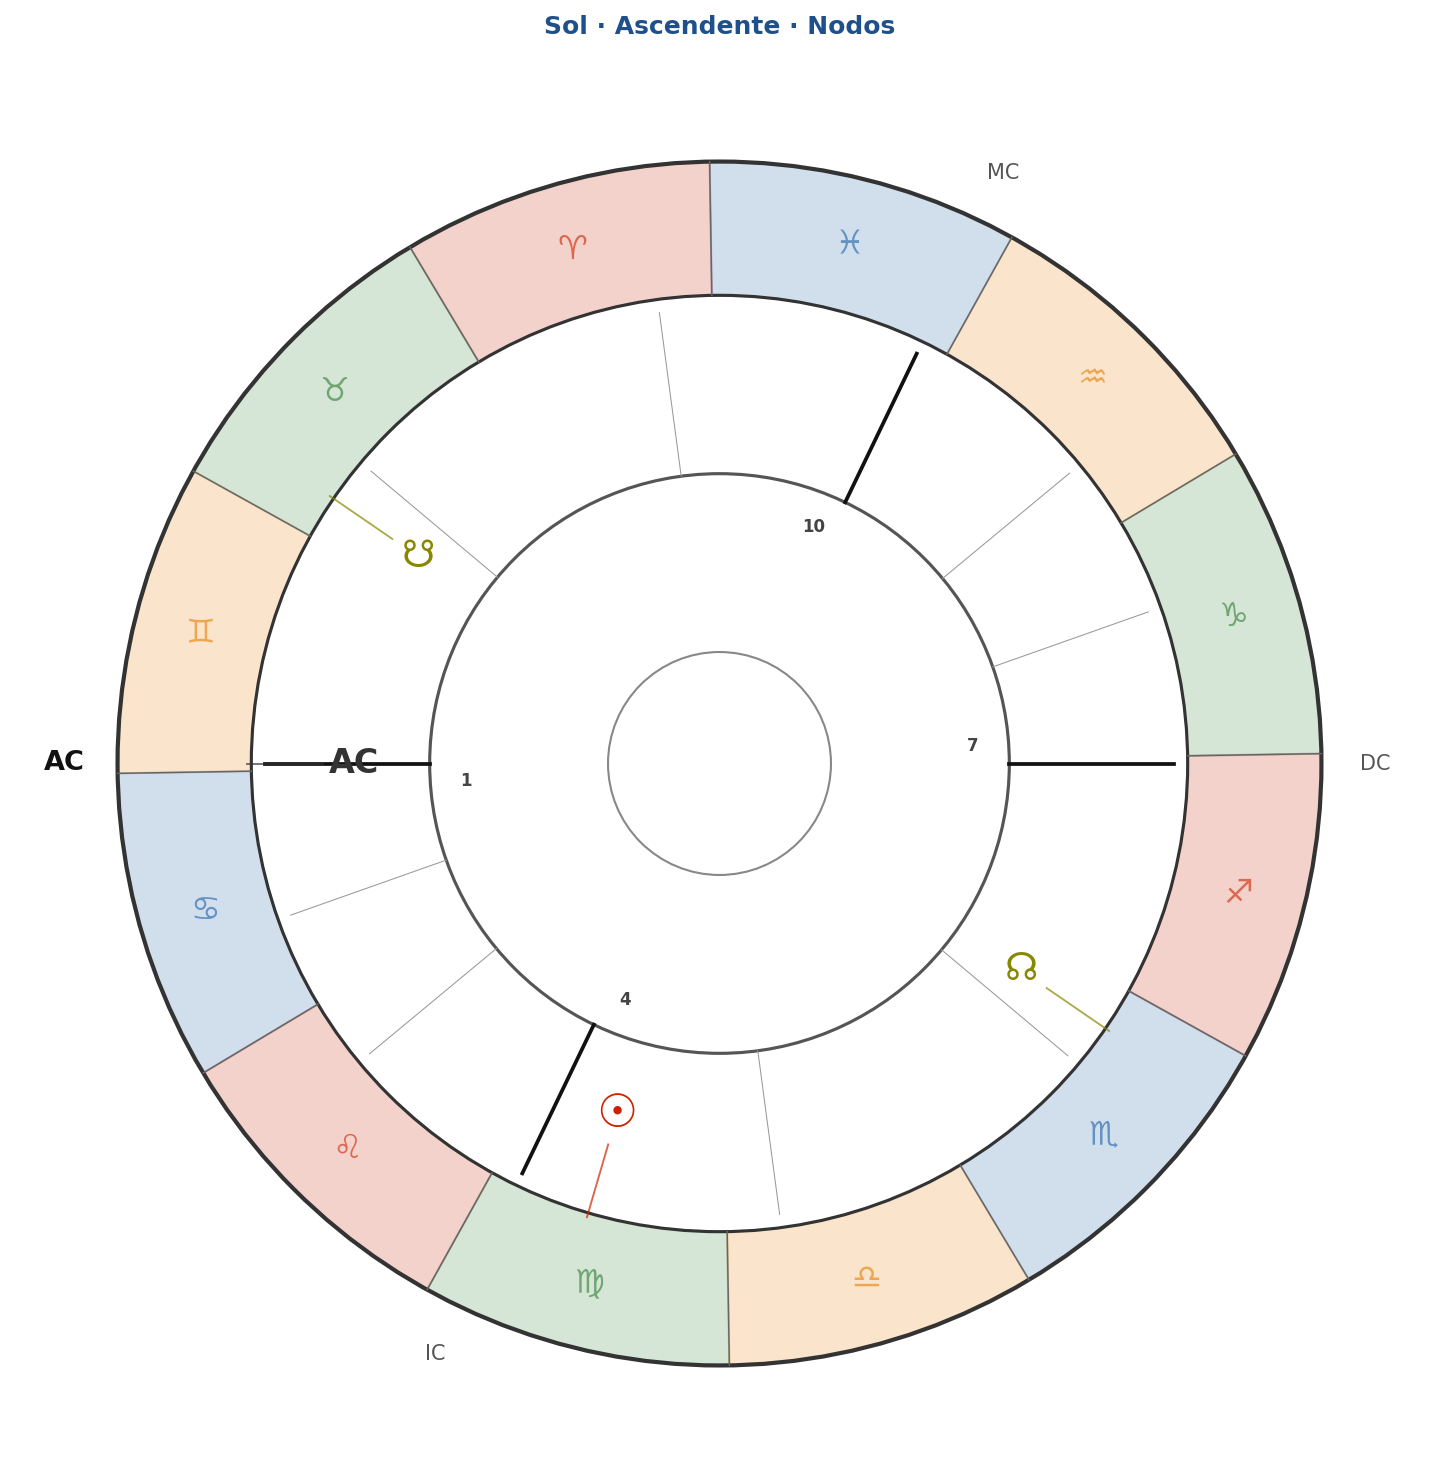
\includegraphics[width=0.72\textwidth]{Virginia_Riezu_Sol_ASC_Nodos_rueda.png}
\end{center}


\vspace{0.3cm}
\Needspace{5\baselineskip}

% ── Interpretación ────────────────────────────────────────────────────────────
\section{Interpretación — Arquitectura Interna}

\begin{center}
{\small\itshape
No se trata de definir quién eres. Se trata de observar cómo se organiza tu dirección,
cómo atraviesas la vida y qué tensión influye en tu forma de avanzar.
}
\end{center}

\vspace{0.5cm}
\Needspace{5\baselineskip}


% ── 1. Dirección general ──────────────────────────────────────────────────────
\needspace{3\baselineskip}
\subsection{1. Dirección general}

El Sol está en Virgo, Casa 4. El Ascendente está en Géminis. El Nodo Norte está en Escorpio, Casa 6, y el Nodo Sur en Tauro, Casa 12.

El Sol en Virgo y el Ascendente en Géminis pertenecen a elementos con lógicas diferentes. Esto puede hacer que vivas las cosas de una forma, mientras otra parte de ti necesita orientarse desde un ritmo completamente diferente.

El Sol en Virgo, Casa 4, no tiene un aspecto directo con los Nodos. La tensión entre el Nodo Norte en Escorpio, Casa 6, y el Nodo Sur en Tauro, Casa 12, se expresa de una forma más independiente respecto a la dirección solar.

\vspace{0.5cm}
\Needspace{5\baselineskip}


% ── 2. Sol ────────────────────────────────────────────────────────────────────
\needspace{3\baselineskip}
\subsection{2. El Sol — Dirección principal}

\needspace{3\baselineskip}
\subsubsection*{Sol en Virgo · Casa 4}

Tu dirección se activa cuando puedes mejorar algo concreto. Necesitas sentir que lo que haces sirve para algo, que aporta orden, claridad o utilidad real.

Sueles orientarte bien cuando puedes distinguir qué funciona y qué no. La confusión sostenida, la falta de criterio o los entornos caóticos tienden a agotarte profundamente.

Cuando no encuentras una aplicación práctica para tu energía, es fácil entrar en exceso de análisis, preocupación o autoexigencia. Necesitas sentir que tu esfuerzo tiene sentido y que puede convertirse en algo tangible.

Tu dirección nace desde la base interna y el espacio privado. Necesitas sentir cierta seguridad emocional y cierta estabilidad íntima para poder avanzar hacia afuera.

Cuando no tienes un lugar donde descansar de verdad o sientes que debes estar constantemente disponible para el exterior, es fácil perder fuerza y replegarte.

Muchas veces necesitas más tiempo que otras personas para aclarar qué quieres realmente. La dirección aparece cuando puedes sostenerte desde dentro.


\vspace{0.5cm}
\Needspace{5\baselineskip}


% ── 3. Ascendente ─────────────────────────────────────────────────────────────
\needspace{3\baselineskip}
\subsection{3. El Ascendente — Forma de relacionarte con la vida}

\needspace{3\baselineskip}
\subsubsection*{Géminis · Regente: Mercurio}

Necesitas movimiento para entender lo que vives. Necesitas pensar, preguntar, hablar o relacionar lo que ocurre con otras ideas para poder entenderlo.

Cuando no puedes expresarte o explorar lo que piensas, la inquietud empieza a crecer por dentro. Es fácil que aparezca ruido mental, dispersión o sensación de tener demasiadas cosas abiertas al mismo tiempo.

Te ayuda poder hablar sobre lo que vives y darle espacio antes de sacar conclusiones demasiado rápido.

El regente del Ascendente es Mercurio, situado en Libra, Casa 5. Mercurio pertenece al mismo elemento que el Ascendente. Esto suele dar continuidad entre tu primera reacción y la forma en que después elaboras lo que ocurre. La Casa 5 muestra un territorio importante desde el que organizas tu forma de entrar en la vida.

\vspace{0.5cm}
\Needspace{5\baselineskip}


% ── 4. Nodos ──────────────────────────────────────────────────────────────────
\needspace{3\baselineskip}
\subsection{4. Nodo Norte y Nodo Sur — Dirección de crecimiento}

\needspace{3\baselineskip}
\subsubsection*{Nodo Norte en Escorpio · Casa 6 \\
Nodo Sur en Tauro · Casa 12}

Tu dirección pide entrar en procesos de transformación reales y aprender a soltar aquello que ya no puede sostenerse de la misma manera. Necesitas desarrollar más capacidad para atravesar cambios profundos sin intentar conservar constantemente lo conocido. Lo familiar suele llevarte hacia la búsqueda de estabilidad, seguridad y control sobre aquello que ya conoces. Puede haber dificultad para dejar atrás situaciones, vínculos o estructuras incluso cuando ya no tienen vida. El reto está en tolerar el cambio sin necesitar todas las garantías antes de moverte. Crecer hacia este Nodo Norte implica aceptar que algunas etapas terminan antes de que exista claridad completa sobre lo siguiente.

Tu dirección pide desarrollar más orden, estructura cotidiana y capacidad de sostener procesos concretos en la realidad diaria. El crecimiento aparece cuando construyes hábitos, cuidas mejor tus ritmos y aprendes a aterrizar las cosas en la vida real en lugar de dejarlas únicamente en intención o posibilidad. El reto suele estar en no perderte constantemente en lo abstracto, en la dispersión o en la sensación de que todo debe permanecer abierto e indefinido.

Tiendes a buscar estabilidad, control sobre lo conocido y seguridad en aquello que puedes sostener de forma concreta. Hay facilidad para conservar, resistir y construir lentamente en el tiempo, pero también dificultad para entrar en cambios profundos cuando implican perder referencias conocidas. Muchas veces aparece tendencia a mantener situaciones, vínculos o estructuras simplemente porque ofrecen sensación de estabilidad o continuidad. El problema surge cuando permanecer en lo seguro se vuelve más importante que reconocer que algo ya necesita transformarse.

Tiendes a replegarte hacia el mundo interno, el aislamiento o la necesidad de escapar del exceso de realidad externa. Hay facilidad para conectar con lo sensible, percibir lo invisible y sostener procesos internos complejos, pero también riesgo de desconectarte demasiado de la acción concreta y de la realidad cotidiana. Muchas veces retirarte puede sentirse más seguro que tomar decisiones claras o asumir límites y dirección definida. El problema aparece cuando el refugio interno se convierte en una forma de evitar movimiento, responsabilidad o presencia en la vida concreta.

\vspace{0.5cm}
\Needspace{5\baselineskip}


% ── 5. Integración ────────────────────────────────────────────────────────────
\needspace{3\baselineskip}
\subsection{5. Integración — Cómo se relacionan las distintas partes}

El Ascendente en Géminis y el Sol en Virgo pertenecen a elementos con lógicas diferentes. Esto puede hacer que una parte de ti quiera vivir las cosas de una forma, mientras otra necesita avanzar desde un ritmo completamente diferente.Cuando no hay espacio para traducir esas dos formas internas, puedes sentir que reaccionas por un lado y deseas orientarte por otro. El trabajo está en no forzarte a elegir una sola parte, sino en aprender a darles un lugar más coherente.

El Ascendente en Géminis y el Nodo Norte en Escorpio pertenecen a elementos con lógicas diferentes. Esto puede hacer que crecer te pida actuar de una manera que no siempre coincide con tu primera reacción. El trabajo está en aprender a no obedecer siempre al primer impulso y dejar espacio a una dirección más nueva.

\vspace{0.5cm}
\Needspace{5\baselineskip}


% ── 6. Orientación práctica ───────────────────────────────────────────────────
\needspace{3\baselineskip}
\subsection{6. Orientación práctica}

\needspace{3\baselineskip}
\subsubsection*{Desde dónde empezar}
Desde el Ascendente en Géminis: poner en palabras lo que está ocurriendo. Hablar sobre ello, escribirlo o compartirlo con alguien puede ayudarte a comprender mejor lo que estás viviendo.

\needspace{3\baselineskip}
\subsubsection*{Qué conviene sostener}
El Sol en Virgo, Casa 4, necesita construir algo concreto y sostenible. Te ayuda avanzar paso a paso y ver que lo que haces va tomando forma.

\needspace{3\baselineskip}
\subsubsection*{Qué conviene observar}
Evita funcionar únicamente desde el Nodo Sur en Tauro, Casa 12. Ese lugar puede resultarte conocido y eficaz, pero no debería convertirse en la única respuesta disponible. La señal de alerta aparece cuando resuelves siempre desde lo que ya sabes hacer, sin preguntarte si esa respuesta sigue siendo adecuada.

El Nodo Norte en Escorpio, Casa 6, pide desarrollar una forma nueva de orientarte, aunque al principio resulte menos automática.

\vspace{1cm}

\begin{center}
{\small\itshape\color{grisai}
La astrología se utiliza aquí como una herramienta de observación y orientación.
No define quién eres ni determina lo que va a ocurrir.
}
\end{center}

\end{document}
